\documentclass{article}
\usepackage[utf8]{inputenc}
\usepackage[T1]{fontenc}
\usepackage{booktabs}
\usepackage{graphicx}
\usepackage[margin=1in]{geometry}

\title{Ablação RGAT vs.\ T5 puro no ScienceBenchmark}
\author{}
\date{}

\begin{document}
\maketitle

\section{Introdução}

Esta nota completa a matriz 2$\times$2 de ablação (tamanho do modelo
$\times$ presença de RGAT) no ScienceBenchmark, complementando
\texttt{docs/sciencebenchmark-eval-results.tex} (t5-small sem RGAT,
t5-base com RGAT completo) e \texttt{estudo/spider\_ablation.tex} (o
mesmo experimento no Spider). Aqui documentamos as duas células que
faltavam: \textbf{t5-base sem RGAT} e \textbf{t5-small com RGAT}
(treinado do zero, sem pré-treino no Spider), ambos com os mesmos dados
e hiperparâmetros (3 épocas, lote efetivo 32, $5\times10^{-5}$ com
adafactor) dos demais fine-tunings no ScienceBenchmark.

\section{Tabela de métricas}

\begin{table}[h]
\centering
\caption{Todas as configurações do ScienceBenchmark, dev set (289/287 exemplos pontuados).}
\label{tab:scibench-ablation}
\begin{tabular}{lrrrrr}
\toprule
\textbf{Configuração} & \textbf{exact match} & \textbf{exec} & \textbf{eval\_loss} & \textbf{train\_loss} & \textbf{tempo de treino} \\
\midrule
t5-small \textbf{sem} RGAT      & 1,38\% & 1,37\% & 1,1825 & 1,0452 & 2h53min \\
t5-small \textbf{com} RGAT       & 1,04\% & 0,68\% & 1,1517 & 0,9977 & 3h46min \\
t5-base \textbf{sem} RGAT        & \textbf{7,27\%} & \textbf{8,19\%} & 0,8010 & 0,5051 & 4h13min \\
t5-base \textbf{com} RGAT (completo, +oncomx, gc) & 0,0\% & 0,34\% & 1,6765 & 2,2152 & 9h42min \\
\bottomrule
\end{tabular}
\end{table}

\section{Achados}

\textbf{1. Tamanho do modelo domina.} t5-base sem RGAT
(7,27\%/8,19\%) é, de longe, a melhor configuração do ScienceBenchmark
inteiro -- superando inclusive o zero-shot com RGAT
(9,0\%/8,87\%\footnote{Ver \texttt{docs/sciencebenchmark-eval-results.tex}, Tabela~1.}
em \emph{exec}, embora ainda um pouco atrás em \emph{exact match}) e
todas as demais tentativas de fine-tuning. Nenhuma configuração
\emph{com} RGAT chega perto: mesmo o melhor caso com RGAT (t5-small,
0,68\% exec) fica mais de 10$\times$ atrás do t5-base sem RGAT.

\textbf{2. RGAT nunca vence sua contraparte do mesmo tamanho.} Com
t5-small controlado (mesmo modelo, mesmos dados, mesmos
hiperparâmetros), \textbf{sem} RGAT vence \textbf{com} RGAT em ambas as
métricas (1,38\%/1,37\% vs.\ 1,04\%/0,68\%) e ainda treina mais rápido
(2h53 vs.\ 3h46 -- RGAT tem o custo computacional extra de construir e
propagar mensagens pelos grafos de até 1300 nós do \texttt{oncomx}).
Esta é a comparação mais controlada de todo o trabalho (mesmo tamanho
de modelo, única variável = presença de RGAT) e o resultado é
inequívoco.

\textbf{3. O padrão se repete em ambos os benchmarks.} A
Figura~\ref{fig:comparison} mostra as quatro curvas de \emph{exec} ao
longo do treino: t5-base sem RGAT destacado muito acima de todas as
outras, que ficam próximas de zero e embaralhadas entre si. Combinado
com \texttt{estudo/spider\_ablation.tex} (onde t5-base sem RGAT também
praticamente empata com o checkpoint RGAT de referência no Spider), a
evidência agora cobre \textbf{quatro} comparações independentes
(2 tamanhos de modelo $\times$ 2 benchmarks) e todas apontam na mesma
direção: dentro do orçamento de treino usado neste trabalho, a
estrutura de grafo do RGAT não demonstrou vantagem sobre um T5 padrão
do mesmo tamanho -- em nenhuma delas.

\begin{figure}[h]
\centering
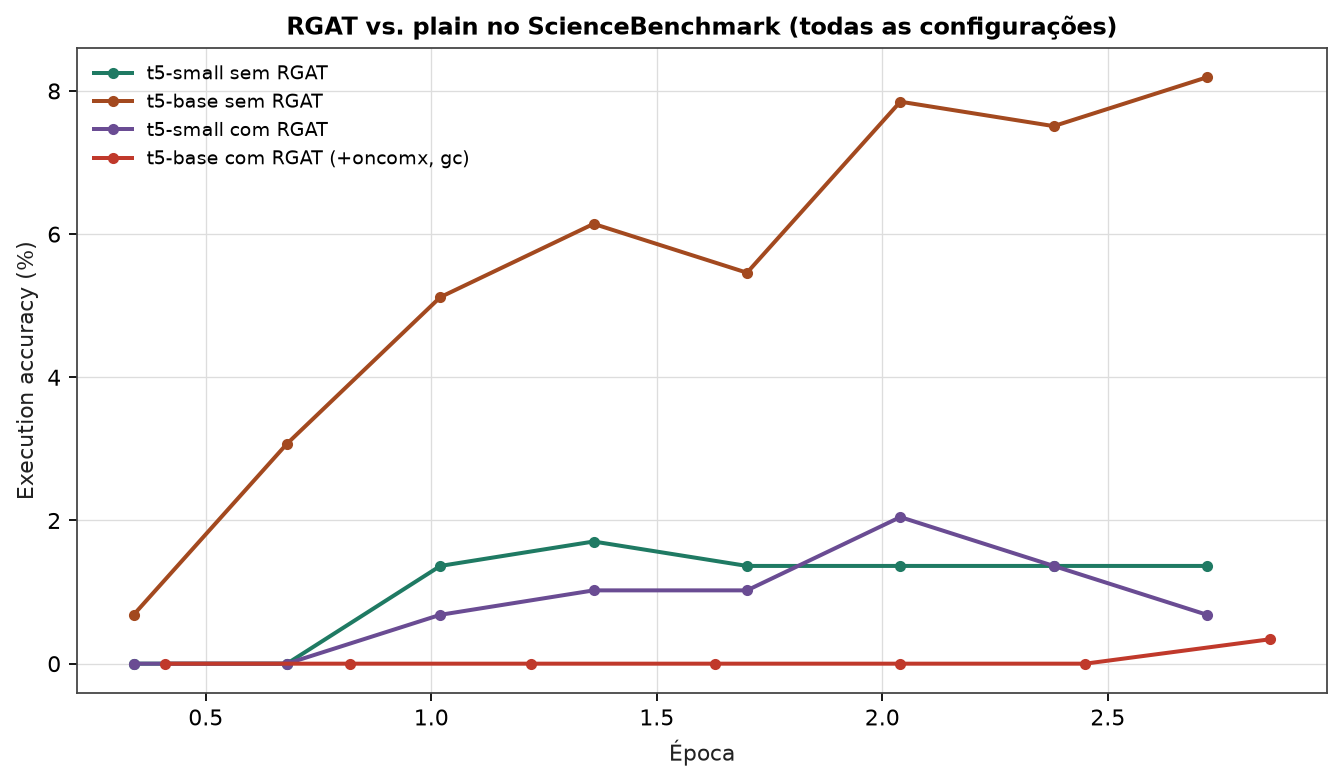
\includegraphics[width=0.95\textwidth]{scibench_ablation_comparison.png}
\caption{Execution accuracy de validação, todas as quatro configurações do ScienceBenchmark.}
\label{fig:comparison}
\end{figure}

\section{Curvas de treino}

\begin{figure}[h]
\centering
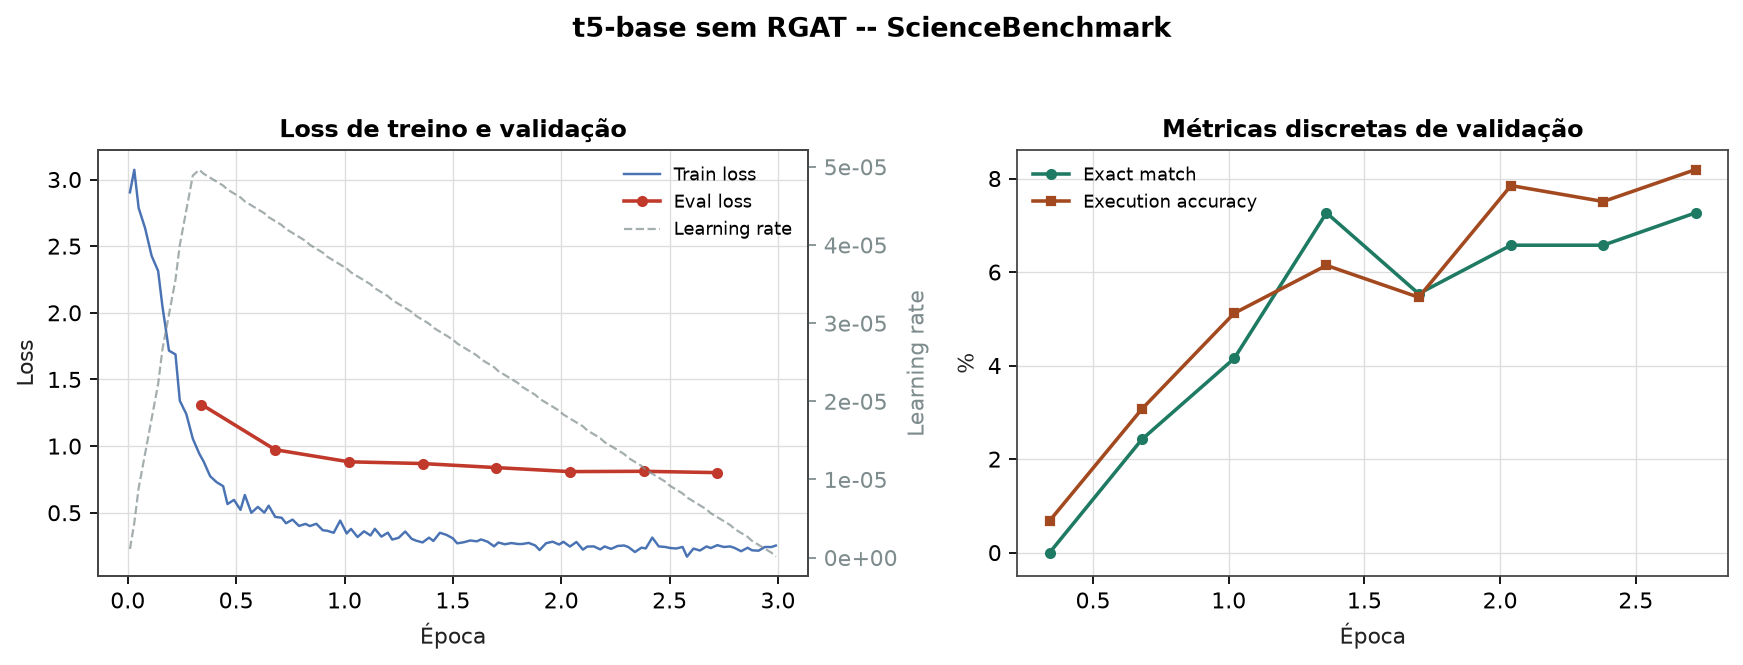
\includegraphics[width=0.95\textwidth]{scibench_t5base_plain_training.png}
\caption{t5-base sem RGAT no ScienceBenchmark -- curvas de treino completas.}
\end{figure}

\begin{figure}[h]
\centering
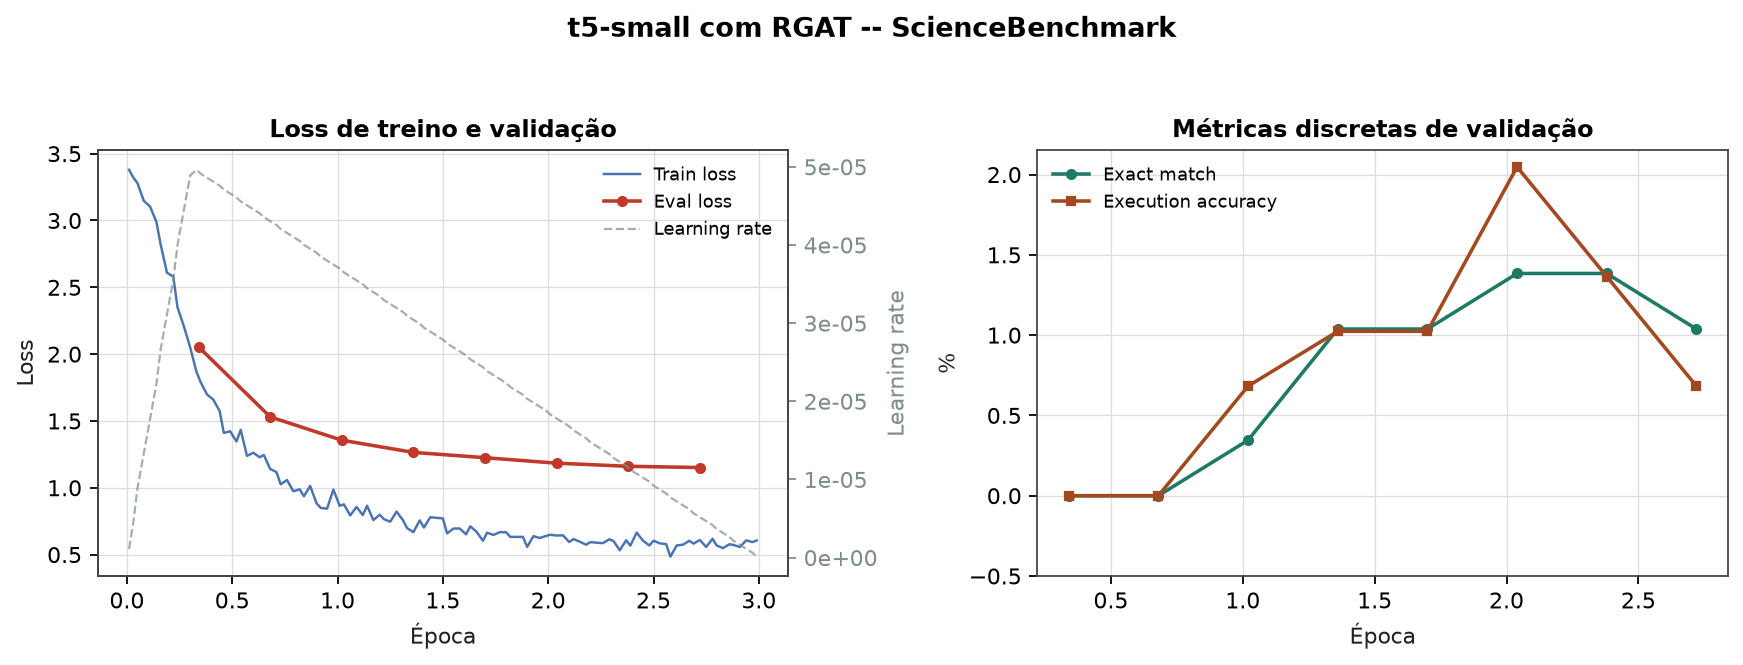
\includegraphics[width=0.95\textwidth]{scibench_t5small_rgat_training.png}
\caption{t5-small com RGAT no ScienceBenchmark -- curvas de treino completas.}
\end{figure}

\end{document}
